\section{Passports}

The protocol governing machine-readable travel documents (MRTD) is Document
9309, issued by the International Civil Aviation Organization
\parencite{ICAO9309}. These standards define the common form that all passports
must take to ensure interoperability. Since all states must operate on a shared
standard, the diplomatic community has forged a compromise between cultural
diversity and international security; the 9309 standard provides sufficient
flexibility to accommodate the diverse languages and scripts used worldwide.

A 9309-compliant MRTD data page is divided into two sections: the Visual
Inspection Zone (VIZ) and the Machine Readable Zone (MRZ).

\subsection{Visual Inspection Zone}

The Visual Inspection Zone, consisting of the top two-thirds of the passport's
data page is designed for inspection by border officials at the point of entry.
States may populate the required VIZ fields in their official language provided
a translation is provided into English, Spanish, or French. Modernized passports
do not \textit{per se} coax a country toward the adoption of standard alphabets;
however, they do ensure effcient intercommunication in the world's
\textit{scripta franca}, the Latin alphabet.

\subsection{Machine Readable Zone}

In contrast, the content of the Machine Readable Zone is highly controlled. The
only characters allowed in the two lines of the MRZ are those belonging to a
defined ASCII subset: (0-9, A-Z, and <). Moreover, these characters must be
printed in the typeface OCR-B (OCR=Optical Character Recognition) using
character and line spacings strictly defined in the 9309 standard. The adherence
to these guidelines allows for unambiguous machine recognition.

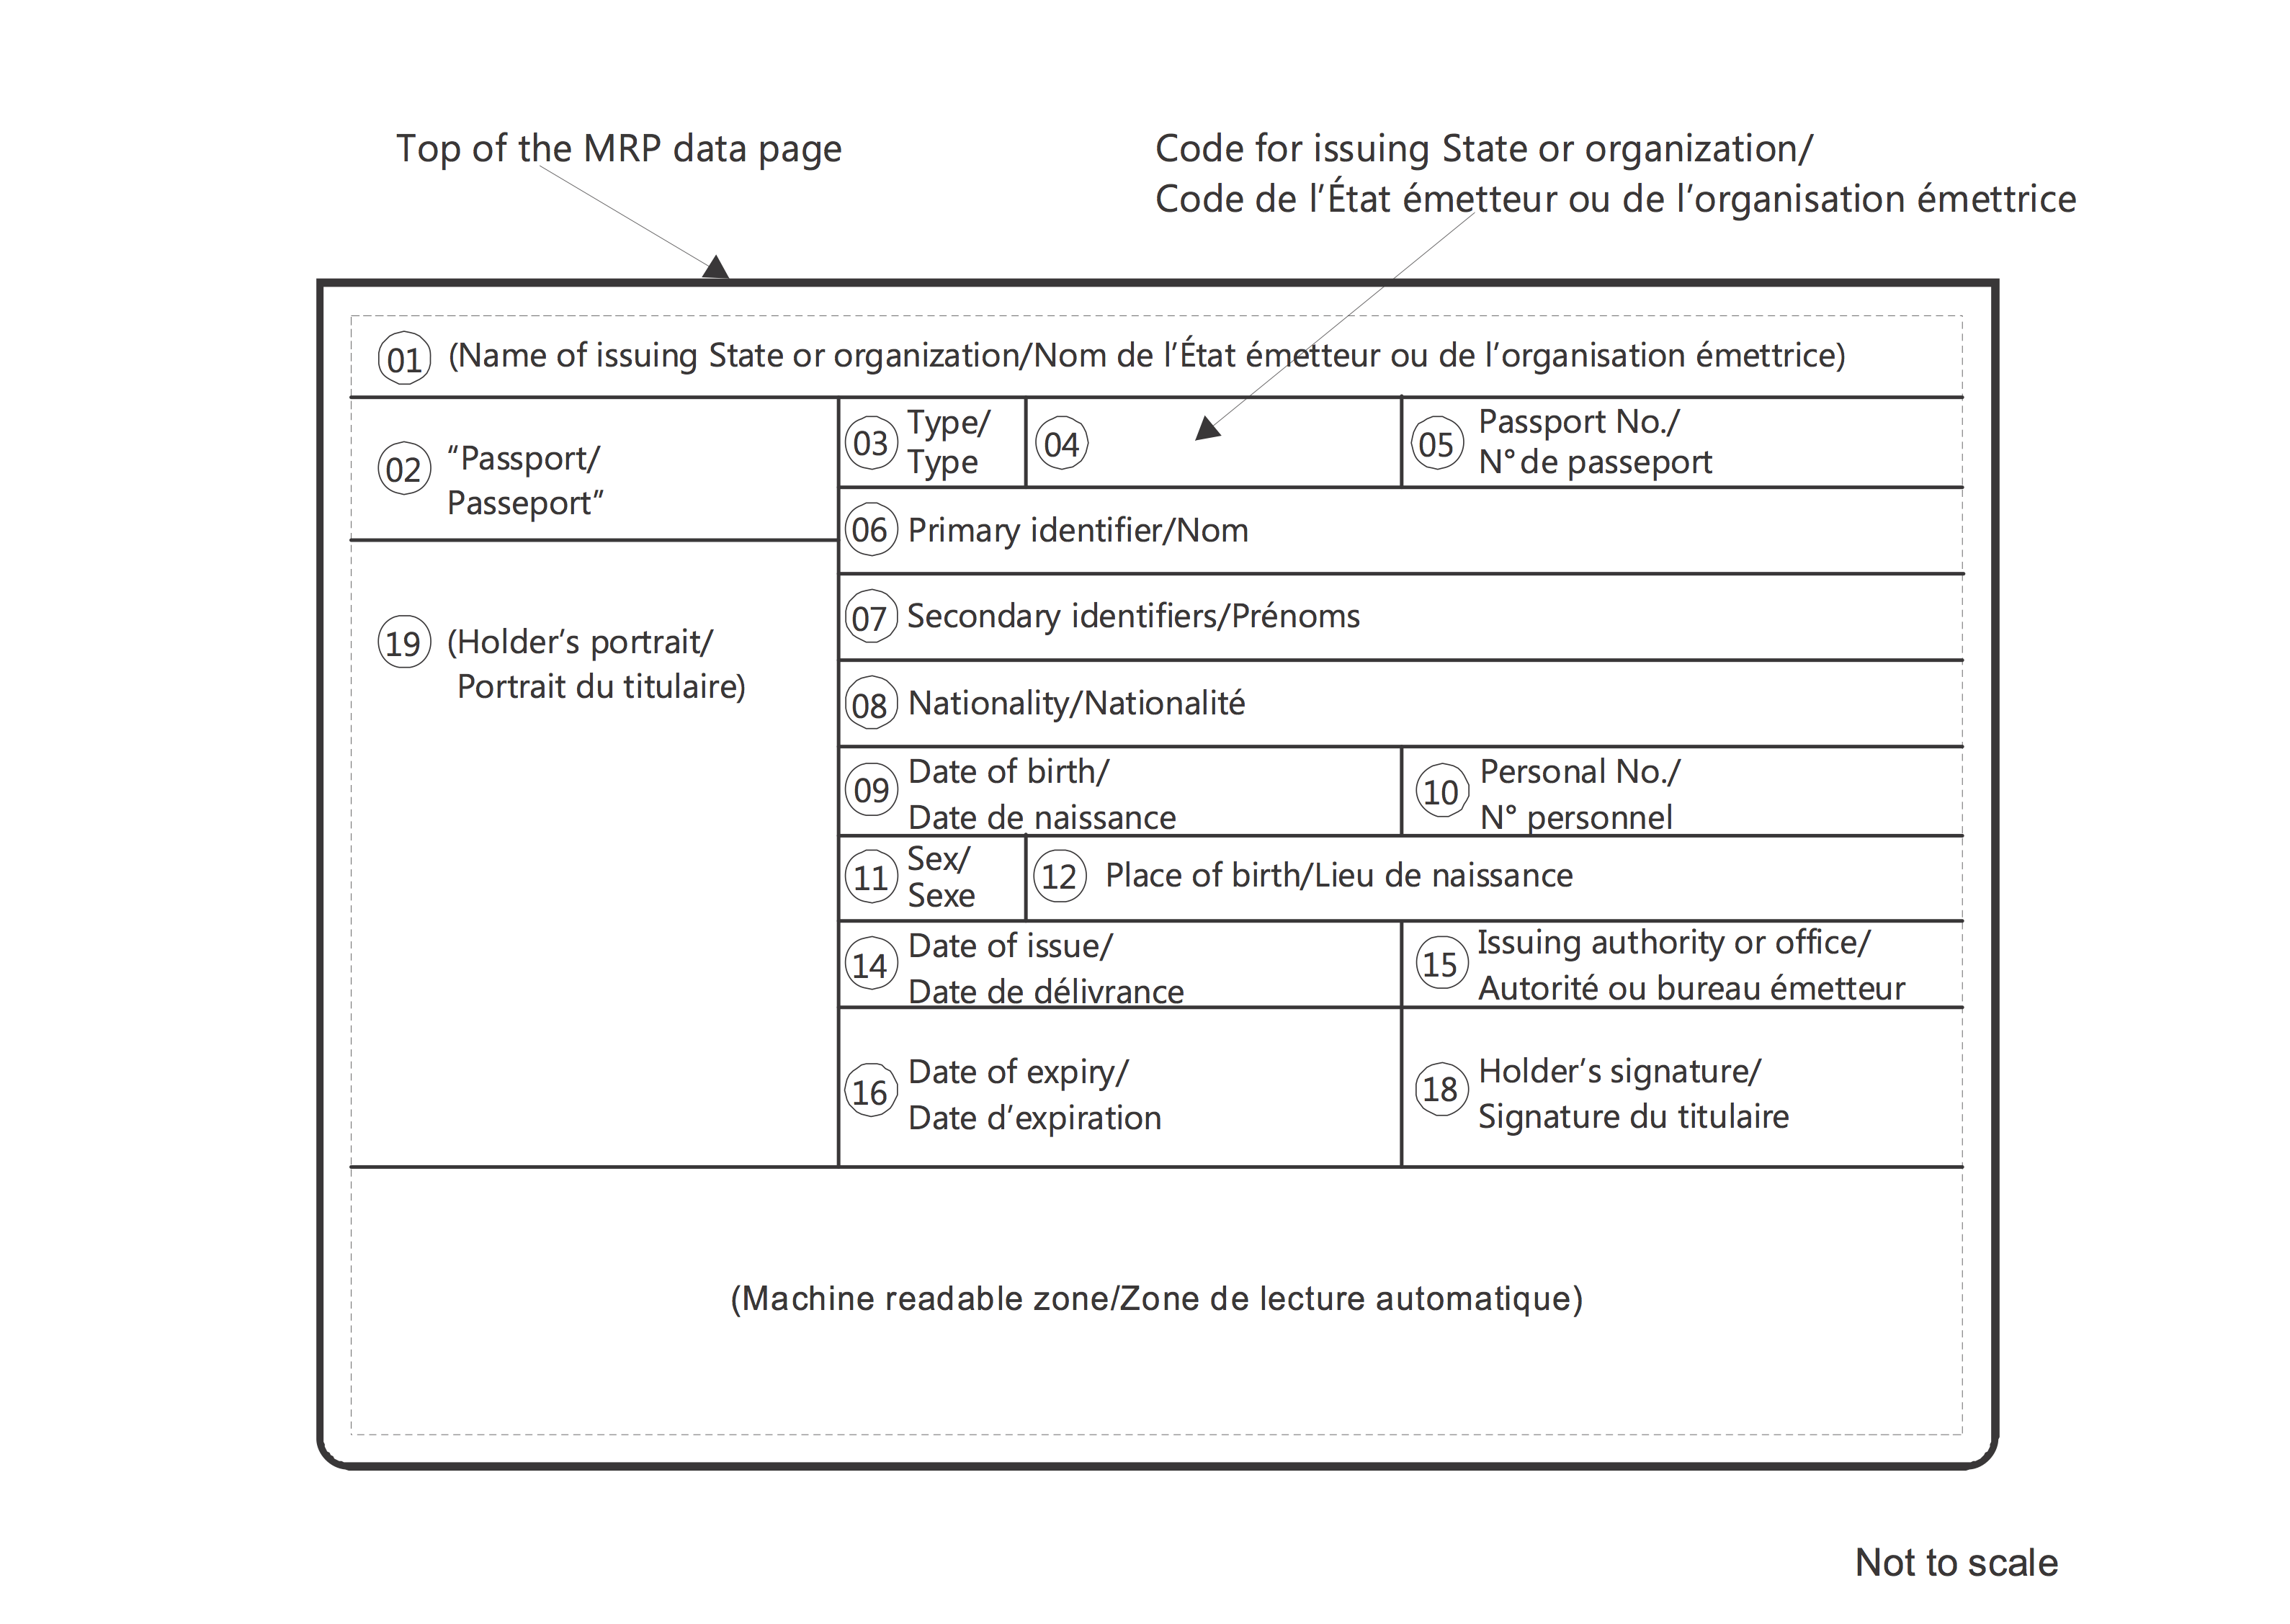
\includegraphics{subtex/9309.4.3.2.4.png}

In the Latin alphabet, most characters with diacritical marks simply have the
mark dropped; some characters, however, do have special encodings to losslessly
transliterate the character. The document provides a more extensive scheme for
the Cyrilic and Arabic scripts, which allows nearly lossless recovery of the
original form from the MRZ content. They even provide a sample Python program
for converting from the MRZ name to Unicode Arabic (\parencite{ICAO9309}
(3.B.7.1).

\subsubsection{Latin}

The ICAO tries to account for the varying importance of diacritical marks in
Latin-based scripts. Those such as the acute or grave accents, which appear over
vowels mainly for the purpose of clarifying pronunciation, are simply eliminated
in the MRZ. However, other characters receive recommended encoding methods These
are the more "salient" diacritic characters, such as the German umlauts (ä, ö,
ü) or the Spanish ñ, which in their respective languages are considered separate
letters, rather than a variation on the unaccented form. The following table
shows the special encodings recommended for European diacritics; all other
characters simply have the mark dropped:

\begin{tabular}{l|l|l|l}
\textbf{Unicode} & \textbf{National Character} & \textbf{Description} &
\textbf{Recommended transliteration} \\
00C4 & Ä & A diaeresis & AE or A \\
00C5 & Å & A ring above & AA or A \\
00C6 & Æ & ligature AE & AE \\
00D1 & Ñ & N tilde & N or NXX \\
00D6 & Ö & O diaeresis & OE or O \\
00D8 & Ø & O stroke & OE \\
00DC & Ü & U diaeresis & UE or UXX or U \\
00DE & Þ & Thorn (Iceland) & TH \\
00DF & ß & double S (Germany) & SS \\
0132 & IJ & ligature IJ (Netherlands) & IJ \\
0152 & Π& ligature OE & OE \\
\end{tabular} (\parencite{ICAO9309} 3.6.A)

The name "Térèsa Cañón" would become CANXXON<<TERESA in the MRZ. The ñ is
encoded in the MRZ, while no distinction is made of the é or è. Likewise, the
German name "Wilhelm Furtwängler" would become FURTWAENGLER<<WILHELM (ä becomes
AE). (b.4.2) Although it leaves a large set of European characters
unrepresented, it would not be difficult to expand the escape sequence system to
represent additional diacritical marks. (An interesting edge case would be a
Spanish traveller named José Nuñenxx.)

\subsubsection{Cyrillic}

The ICAO transcription system for Cyrillic characters permits a nearly
one-to-one transliteration between the MRZ and the name in the original
language. The system recognizes the different values that a Cyrillic glyph might
take in various languages. For example the letter Ю is transliterated as "IU",
unless it is the first character of a Ukrainian name, in which case "YU" is
permitted. Likewise for Щ; this is SHCH, except in Bulgarian, where it is SHT.

\subsubsection{Arabic}

For example, the Arabic name {\arfont ابو بكر محمد بن زكريا الرازي} would be
rendered in the MRZ as ABW<BKR<MXHMD<<BN<ZKRYA<ALRAZY.

While the name looks incomprehensible to a human, the encoding permits a
one-to-one mapping between the MRZ and the original Arabic name. See more
examples in the figure below:

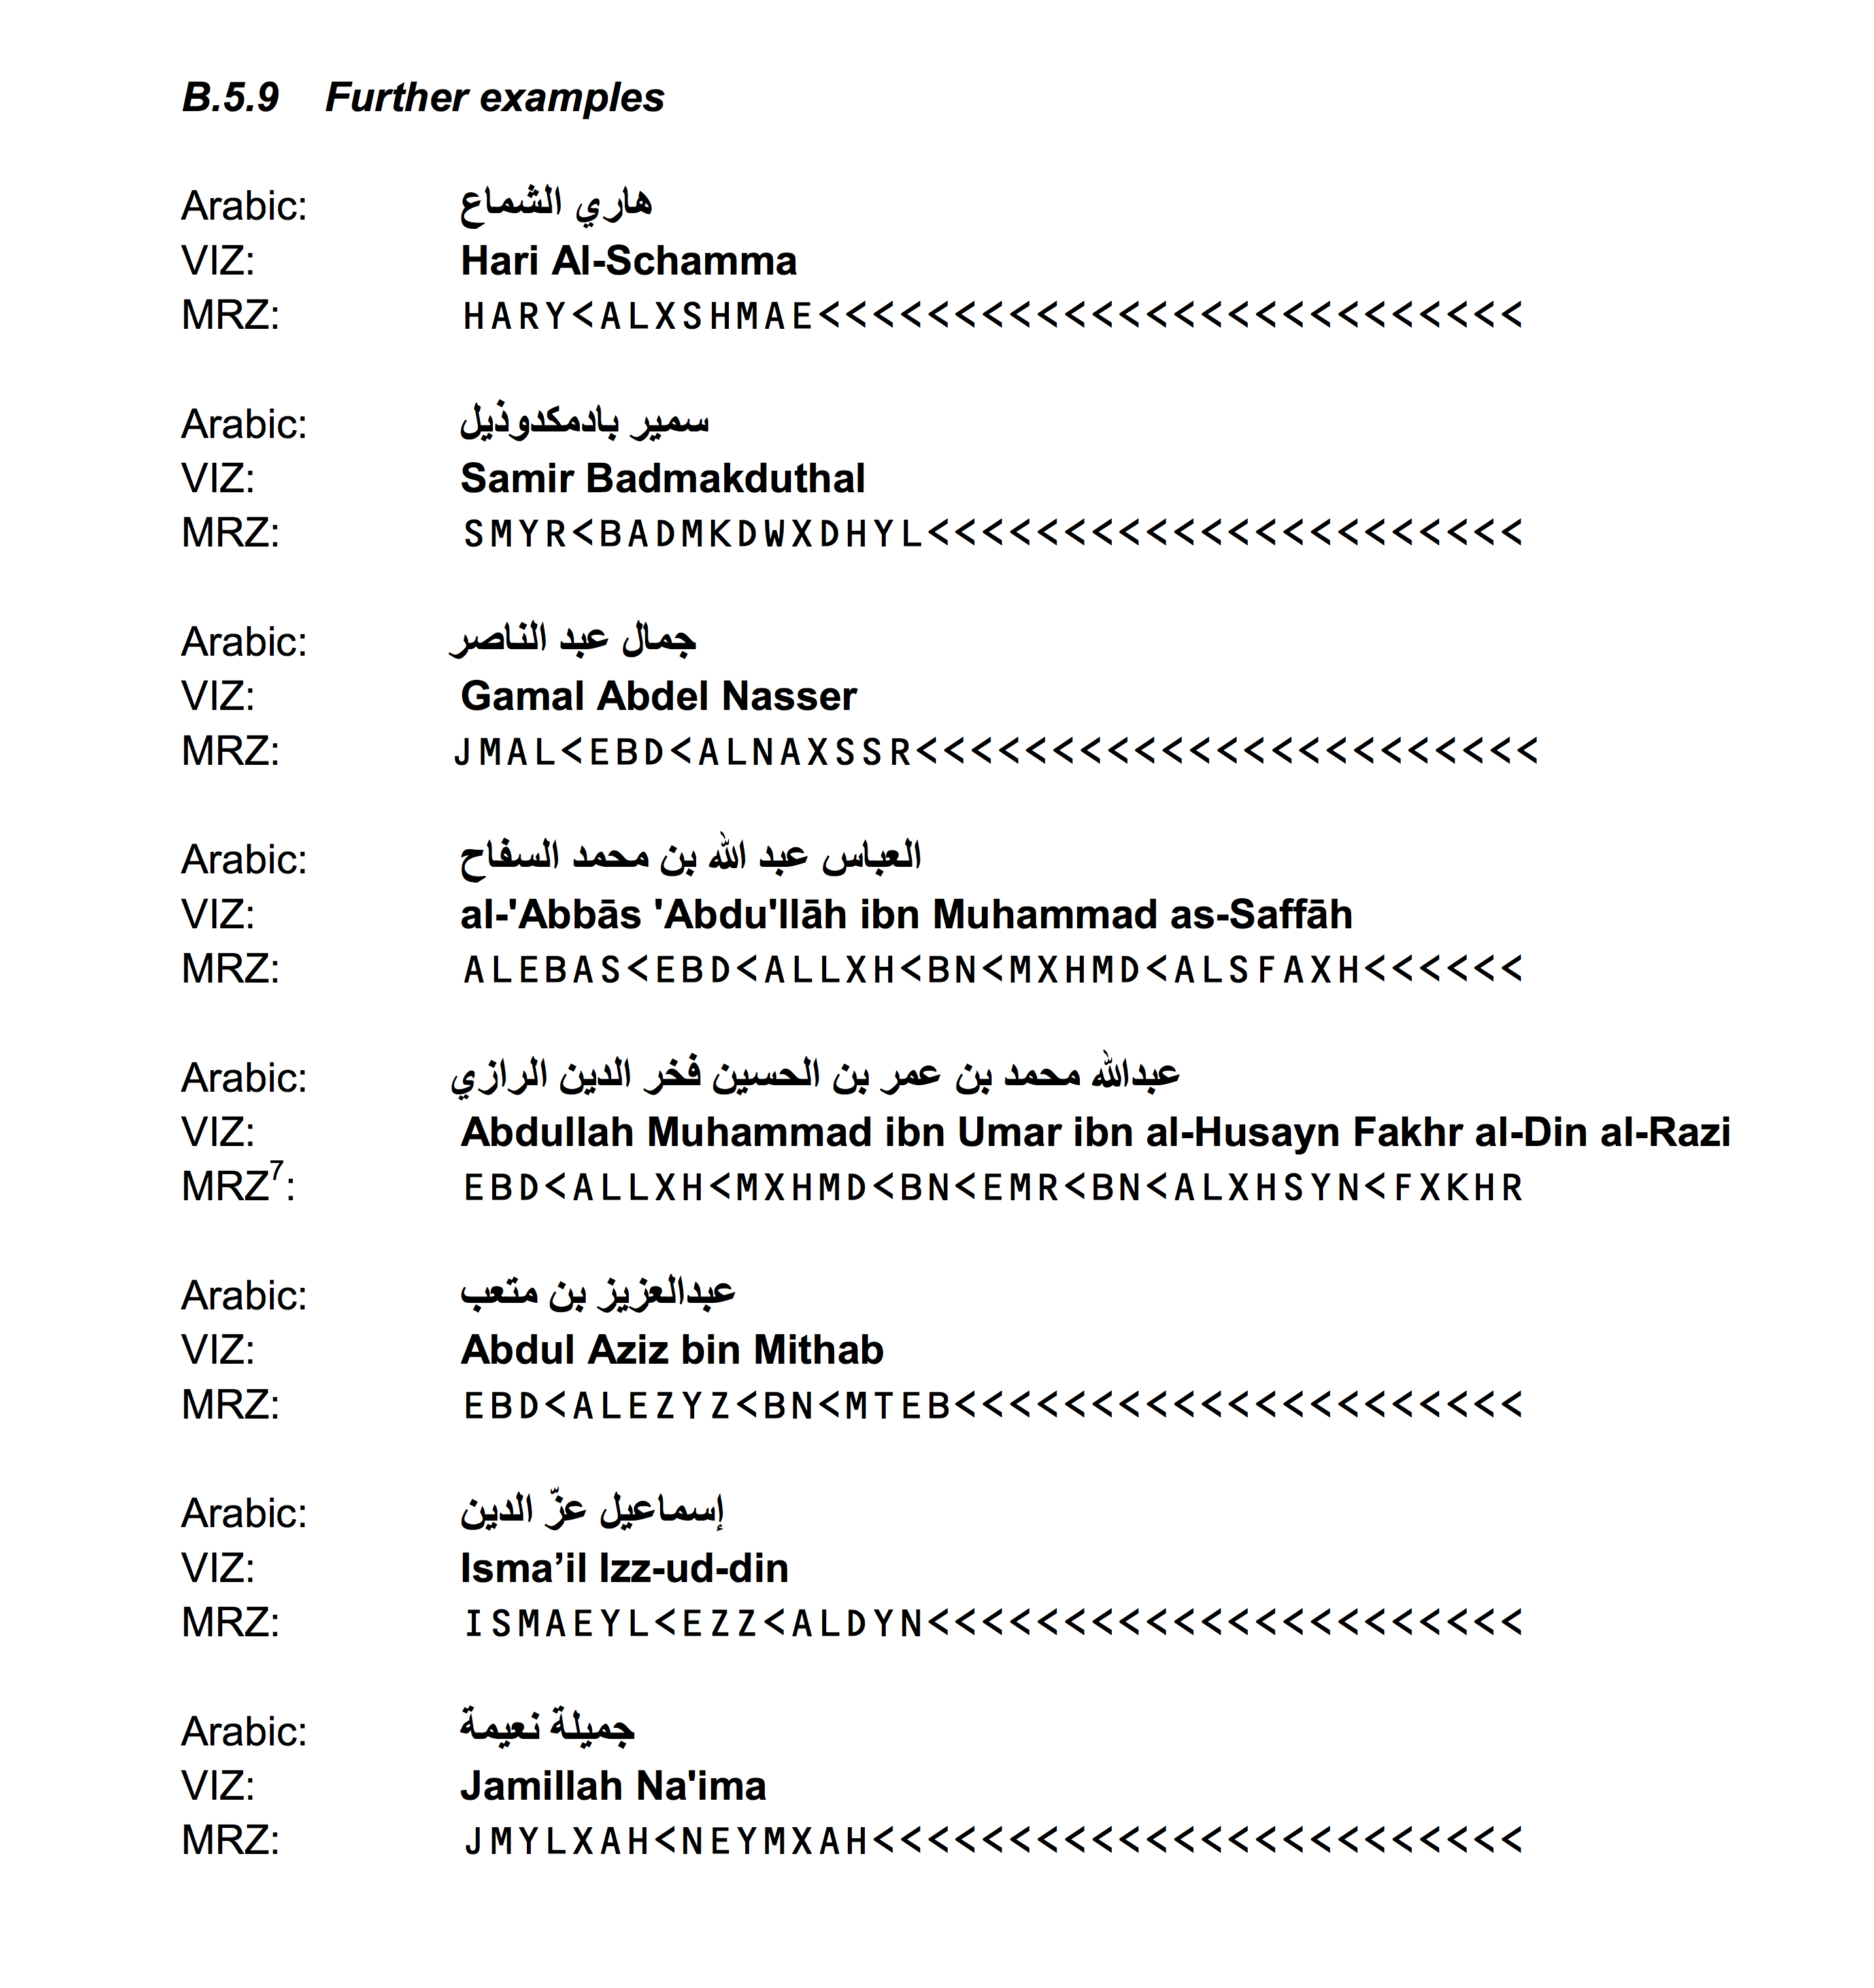
\includegraphics{subtex/9309.3-appendix-b.5.9.png}
